\chapter*{Appendix: Comparison of results of direct render implementations}
\addcontentsline{toc}{chapter}{Appendix}

In this appendix, we present comparison of results between fixed direct renderer \; implementation as defined in equation \ref{eq:sengupta-direct-fix} and our own implementation using physically correct Phong BRDF. As we can see in figure \ref{fig:comparison-direct}, due to inclusion of specular albedo and glossiness into the implementation, we can render much better images that are more similar to the original image. Images were rendered with an environment map inferred by our trained EnvMap model and ground-truth data for each scene.
\begin{figure}[H]
    \centering
    \begin{subfigure}{0.32\linewidth}
        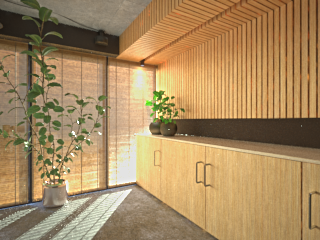
\includegraphics[width=\linewidth]{praca/images/AI53_020_Cam09.png}
    \end{subfigure}
    \begin{subfigure}{0.32\linewidth}
        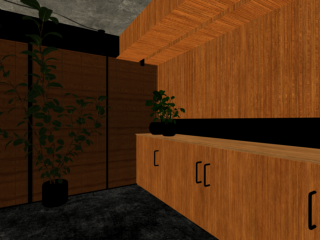
\includegraphics[width=\linewidth]{praca/images/AI53_020_Cam09.direct_sengputa.png}
    \end{subfigure}
    \begin{subfigure}{0.32\linewidth}
        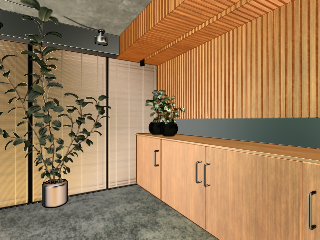
\includegraphics[width=\linewidth]{praca/images/AI53_020_Cam09.direct_ours.png}
    \end{subfigure}
    \begin{subfigure}{0.32\linewidth}
        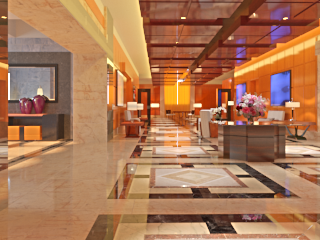
\includegraphics[width=\linewidth]{praca/images/AI44_010_Cam01.png}
    \end{subfigure}
    \begin{subfigure}{0.32\linewidth}
        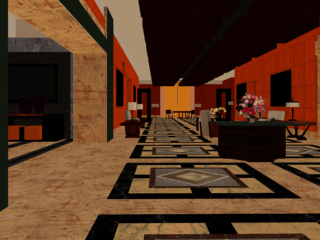
\includegraphics[width=\linewidth]{praca/images/AI44_010_Cam01.direct_sengputa.png}
    \end{subfigure}
    \begin{subfigure}{0.32\linewidth}
        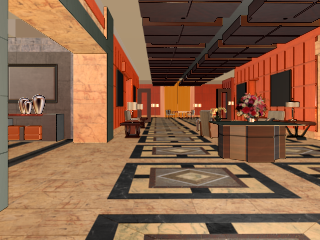
\includegraphics[width=\linewidth]{praca/images/AI44_010_Cam01.direct_ours.png}
    \end{subfigure}
    \begin{subfigure}{0.32\linewidth}
        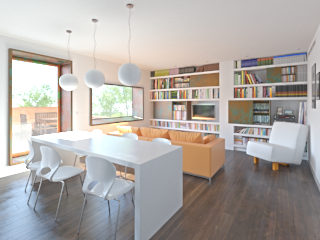
\includegraphics[width=\linewidth]{praca/images/AI45_002_Cam01.png}
    \end{subfigure}
    \begin{subfigure}{0.32\linewidth}
        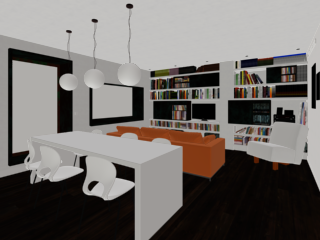
\includegraphics[width=\linewidth]{praca/images/AI45_002_Cam01.direct_sengputa.png}
    \end{subfigure}
    \begin{subfigure}{0.32\linewidth}
        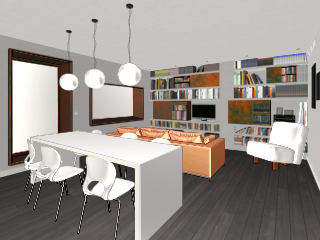
\includegraphics[width=\linewidth]{praca/images/AI45_002_Cam01.direct_ours.png}
    \end{subfigure}
    \caption[Comparison of direct render results]{Comparison of direct render results, with original image (left), image rendered by original direct render implementation (middle) and image rendered by our own implementation of direct render (right)}
    \label{fig:comparison-direct}
\end{figure}
